%\documentclass[tikz, convert]{standalone}
\documentclass[
  tikz, convert={density=800, size=2600x1300}, 
  background, border=0.5cm
 ]{standalone}
\usetikzlibrary{shapes.geometric, positioning}
\usetikzlibrary{quotes, angles, calc, backgrounds}

\tikzset{decisionNode/.style={inner sep=5pt, shape=circle,align=center,font=\Large,draw, fill=gray!40}}
\tikzset{leafNode/.style={inner sep=5pt, shape=circle, align=center, font = \Large, draw, fill=white}}
\tikzset{decisionRule/.style={shape=rectangle, align=center, font = \normalsize, draw=none, fill=white}}
\tikzset{jump/.style={shape=rectangle, align=center, font=\Large, draw=none, fill=white}}
\tikzset{annotation/.style={shape=rectangle, align=center, font=\Large, draw=none, fill=white}}


%%
% label placement:
% https://tex.stackexchange.com/questions/333282/how-to-put-text-above-a-node-point-in-tikz

% level spacings to avoid overlaps
% https://tex.stackexchange.com/questions/86919/tikz-tree-without-overlaps


\begin{document}



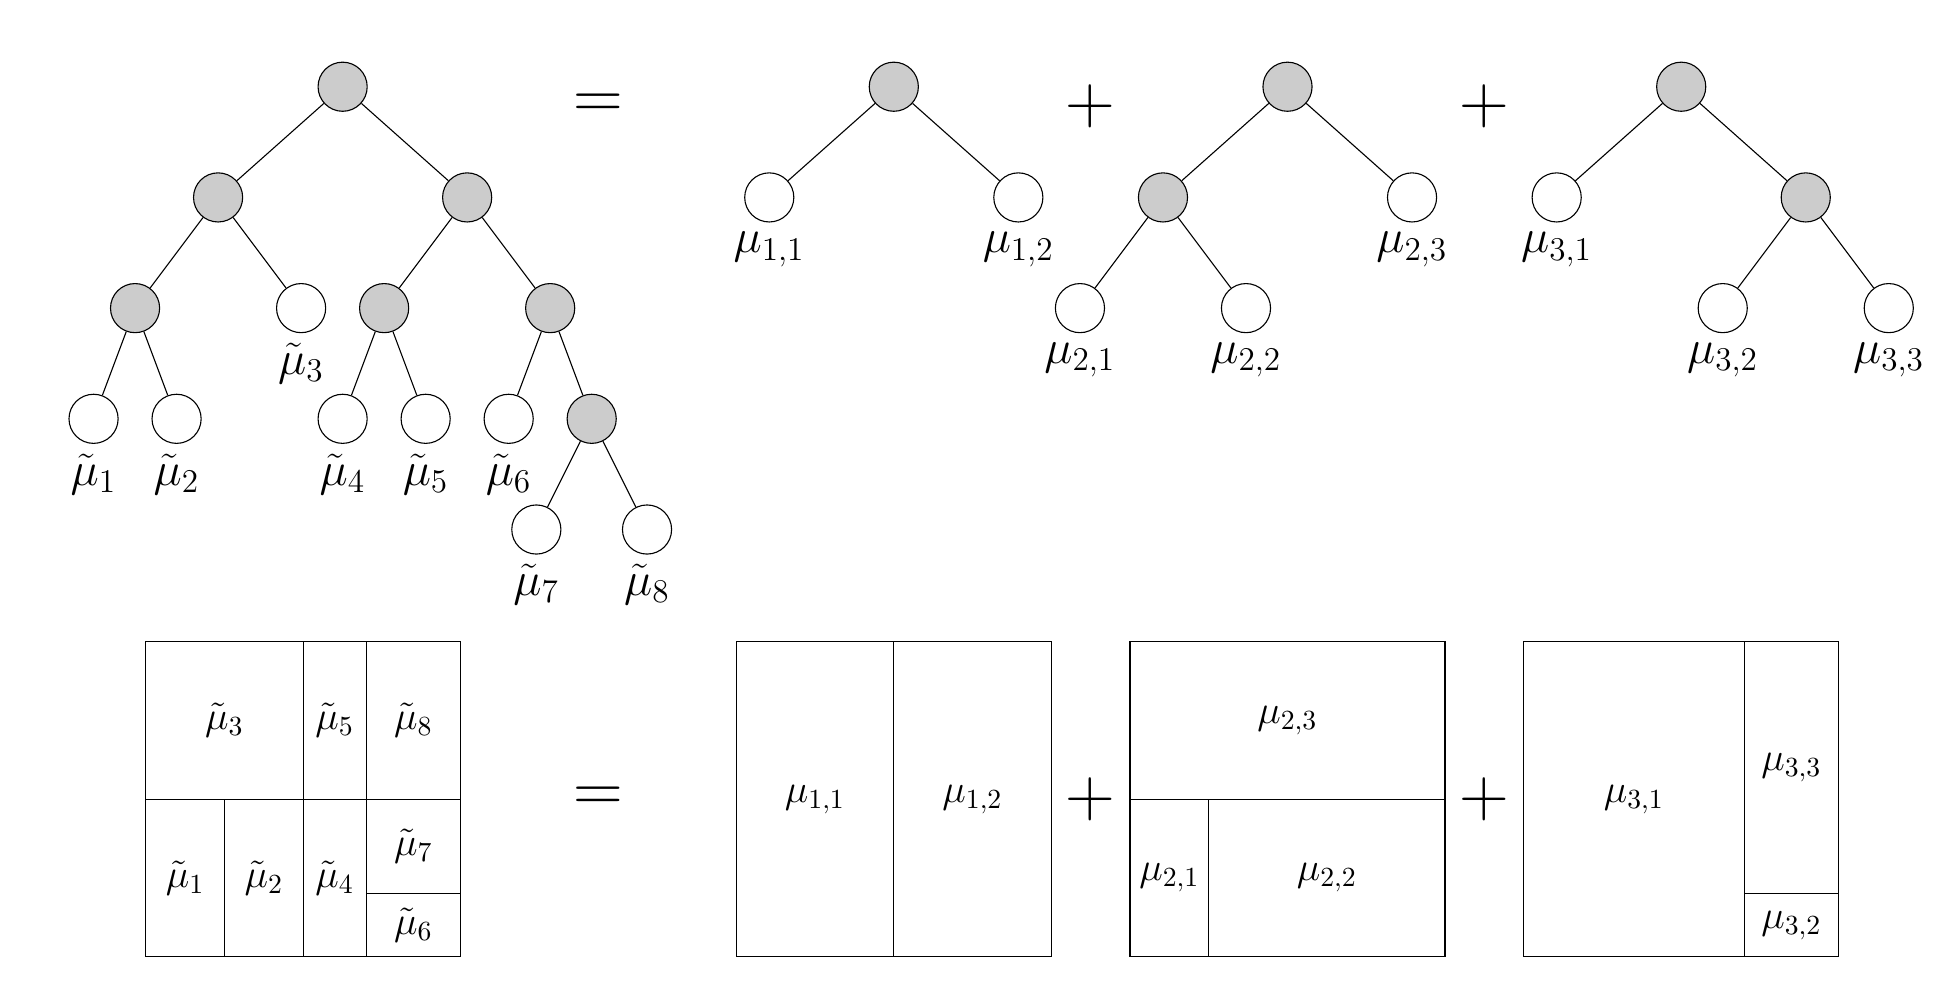
\begin{tikzpicture}[
  background rectangle/.style={fill=white}, show background rectangle,
  level 1/.style={sibling distance = 9em},
  level 2/.style={sibling distance = 6em},
  level 3/.style={sibling distance = 3em},
  level 4/.style={sibling distance = 4em},
  level distance = 4em]
  %sibling distance = 4em, level distance = 4em]
  %sibling distance=4em, level distance = 4em]

\useasboundingbox (-12,-6) rectangle (12,6);
%\draw (0,0) -- (1,0) -- (1,1) -- (0,1) -- (0,0);
\node[decisionNode] (01) at (-8,5.25) {~}
  child{ % child of 1
    node[decisionNode] (02) {~}
    child{ node[decisionNode] (04) {~} 
      child{ node[leafNode, label=below:{\LARGE $\tilde{\mu}_{1}$}] (08) {~}}
      child{ node[leafNode, label=below:{\LARGE $\tilde{\mu}_{2}$}] (09) {~}}
    }
    child{ node[leafNode, label=below:{\LARGE $\tilde{\mu}_{3}$}] (05) {~} }
  }  % end of subtree of 2
  child{node[decisionNode] (03) {~}
    child{node[decisionNode] (06) {~}
    %child{node[decisionNode, label={[label distance=0.2em]92:{\Large$(2, .5)$}}] (06) {~}
      child{node[leafNode, label=below:{\LARGE $\tilde{\mu}_{4}$}] (012) {~}}
      child{node[leafNode, label=below:{\LARGE $\tilde{\mu}_{5}$}] (013) {~}}
    } % end of subtree of 6
    child{node[decisionNode] (07) {~}
      child{node[leafNode, label=below:{\LARGE $\tilde{\mu}_{6}$}] (014) {~} }
      child{node[decisionNode] (015) {~}
        child{node[leafNode, label=below:{\LARGE$\tilde{\mu}_{7}$}] (030) {~}}
        child{node[leafNode, label=below:{\LARGE$\tilde{\mu}_{8}$}] (031) {~}}
      } % end of subtree of 15
    } % end of subtree of 7
  } % end of subtree of 3
;


% Partition version of Tree 0
\draw (-10.5,-5.8) rectangle (-6.5,-1.8);
\draw (-10.5,-5.8) rectangle (-9.5, -3.8) node[pos=0.5]{\Large $\tilde{\mu}_{1}$};
\draw (-9.5, -5.8) rectangle (-8.5, -3.8) node[pos=0.5]{\Large $\tilde{\mu}_{2}$};
\draw (-10.5,-3.8) rectangle (-8.5, -1.8) node[pos=0.5]{\Large $\tilde{\mu}_{3}$};
\draw (-8.5, -5.8) rectangle (-7.7, -3.8) node[pos = 0.5]{\Large $\tilde{\mu}_{4}$};
\draw (-8.5, -3.8) rectangle (-7.7, -1.8) node[pos =0.5]{\Large $\tilde{\mu}_{5}$};
\draw (-7.7,-5.8) rectangle (-6.5, -5) node[pos=0.5]{\Large $\tilde{\mu}_{6}$};
\draw (-7.7, -5) rectangle (-6.5, -3.8) node[pos=0.5]{\Large $\tilde{\mu}_{7}$};
\draw (-7.7, -3.8) rectangle (-6.5, -1.8) node[pos=0.5]{\Large $\tilde{\mu}_{8}$};

%Tree 1
\node[decisionNode] (11) at (-1,5.25) {~}
  child{ node[leafNode, label=below:{\LARGE $\mu_{1,1}$}] (12) {~}}
  child{ node[leafNode, label=below:{\LARGE $\mu_{1,2}$}] (13) {~}}
;

% Partition version of Tree 1
\node[annotation] (equal) at (-4.75, 5) {\Huge $=$};
\node[annotation] (equal) at (-4.75, -3.8) {\Huge $=$};
\draw (-3,-5.8) rectangle (1,-1.8);
\draw (-3,-5.8) rectangle (-1,-1.8) node[pos = 0.5] {\Large $\mu_{1,1}$};
\draw (-1,-5.8) rectangle (1,-1.8) node[pos = 0.5]{\Large $\mu_{1,2}$};

% Tree 2
\node[decisionNode] (21) at (4,5.25) {~}
  child{ node[decisionNode] (22) {~}
    child{ node[leafNode, label=below:{\LARGE $\mu_{2,1}$}] (24) {~} }
    child{ node[leafNode, label=below:{\LARGE $\mu_{2,2}$}] (25) {~} }
  } % closes sub-tree of node 2
  child{ node[leafNode, label=below:{\LARGE $\mu_{2,3}$}] (23) {~}
  }
;

% Partition version of Tree 2
\node[annotation] (plus2) at (1.5, -3.8) {\Huge $+$};
\node[annotation] (plus2) at (1.5, 5) {\Huge $+$};

\draw (2,-5.8) rectangle (6,-1.8);
\draw (2, -5.8) rectangle (3, -3.8) node[pos=0.5]{\Large $\mu_{2,1}$};
\draw (3,-5.8) rectangle( 6, -3.8) node[pos=0.5]{\Large $\mu_{2,2}$};
\draw (2,-3.8) rectangle (6, -1.8) node[pos=0.5]{\Large $\mu_{2,3}$};


% Tree 3
\node[decisionNode] (31) at (9,5.25) {~}
  child{ node[leafNode, label=below:{\LARGE $\mu_{3,1}$}] (32) {~}}
  child{ node[decisionNode] (33) {~}
    child{ node[leafNode, label=below:{\LARGE $\mu_{3,2}$}] (34) {~}}
    child{ node[leafNode, label=below:{\LARGE $\mu_{3,3}$}] (35) {~}}
  }
;
\node[annotation] (plus3) at (6.5, -3.8) {\Huge$+$};
\node[annotation] (plus3) at (6.5, 5) {\Huge$+$};

% Partition version of Tree 3
\draw (7,-5.8) rectangle (11,-1.8);
\draw (7,-5.8) rectangle (9.8,-1.8) node[pos=0.5]{\Large $\mu_{3,1}$};
\draw (9.8,-5.8) rectangle (11,-5) node[pos=0.5]{\Large $\mu_{3,2}$};
\draw (9.8, -5) rectangle (11,-1.8) node[pos=0.5]{\Large $\mu_{3,3}$};


%%% Define the tilde mu
%\node[annotation] at (1,0.9) {\LARGE $\tilde{\mu}_{1} = \mu_{1,1} + \mu_{2,1} + \mu_{3,1}$};
%\node[annotation] at (1,0.2) {\LARGE $\tilde{\mu}_{2} = \mu_{1,1} + \mu_{2,2} + \mu_{3,1}$};
%\node[annotation] at (1,-0.5) {\LARGE $\tilde{\mu}_{3} = \mu_{1,1} + \mu_{2,3} + \mu_{3,1}$};
%\node[annotation] at (1,-1.2) {\LARGE $\tilde{\mu}_{4} = \mu_{1,2} + \mu_{2,2} + \mu_{3,1}$};

%\node[annotation] at (7,0.9) {\LARGE $\tilde{\mu}_{5} = \mu_{1,2} + \mu_{2,3} + \mu_{3,1}$};
%\node[annotation] at (7,0.2) {\LARGE $\tilde{\mu}_{6} = \mu_{1,2} + \mu_{2,2} + \mu_{3,2}$};
%\node[annotation] at (7,-0.5) {\LARGE $\tilde{\mu}_{7} = \mu_{1,2} + \mu_{2,2} + \mu_{3,3}$};
%\node[annotation] at (7,-1.2) {\LARGE $\tilde{\mu}_{8} = \mu_{1,2} + \mu_{2,3} + \mu_{3,3}$};

\end{tikzpicture}

\end{document}